% TODOS
% Does J need to be normalized, wrt Rindler and Minkowski
% Work out details of Green's function
\documentclass[12pt,a4paper]{article}
\usepackage[width=.75\textwidth]{caption}
\usepackage{graphicx}
\usepackage{authblk}
\usepackage{amsmath}
\usepackage{amsfonts}
\usepackage{braket}
\usepackage{epigraph}
%\usepackage{mathrsfs}
\usepackage[mathscr]{euscript}
\usepackage[top=2cm, bottom=2cm, left=2cm, right=2cm]{geometry}
\usepackage{fancyhdr}
\newcommand{\dv}[1]{\mathrm{d} #1 \text{ }}
\newcommand*\diff{\mathop{}\!\mathrm{d}}
\newcommand\restr[2]{{% we make the whole thing an ordinary symbol
  \left.\kern-\nulldelimiterspace % automatically resize the bar with \right
  #1 % the function
  \vphantom{\big|} % pretend it's a little taller at normal size
  \right|_{#2} % this is the delimiter
  }}
\setlength{\epigraphwidth}{0.8\textwidth}

% \pagestyle{fancy}
\begin{document}

%title and author details
\title{Localized Driving and the Role of Thrust in Unruh Radiation}
\author[1]{Kevin Player\footnote{kplaye@gmail.com}}

\maketitle

\epigraph{The Unruh effect tells us that what we call particles is really just a matter of perspective.}{Lee Smolin}

\abstract{We analyze Unruh radiation, interpreting the radiation as sourced by a driving field. In the Rindler frame, the driving modes extend over long durations and experience redshift and blueshift due to their extended support across the wedge, leading to a mixed-frequency response interpreted thermally.  To refine this picture, we construct an interpolation between these long-lived driving modes and localized wave packets with peaked Fourier spectra that do not display such frequency smearing. This allows us to reinterpret Unruh radiation in terms of thrust, a localized driving effect that excites the field without inducing a thermal response, thereby offering a complementary, nonthermal perspective on acceleration-induced radiation.}

\section{Introduction}
We first present some notation and review the Unruh effect in section 2.  We then introduce a source in section 3 that exactly captures the particle creation in the cross term of the Bogoliubov transform for Rindler modes extended to Minkowski space.  In section 4,  we interpolate between the eternal Rindler mode source to a more localized wave packet version, and in section 5 we interpret the results.

\section{Unruh Effect Review and Notation}

We draw notation and standard results from Frodden and Vald{\'{e}}s \cite{Frodden}.


Let $\hbar$ = $c$ = 1. We consider a uniformly accelerating observer in 1+1 dimensional Minkowski spacetime with metric signature $\eta=(-1,+1)$. The extension to 1+3 dimensions does not affect the key physics of the Unruh effect, so we restrict to the (t,x) plane where the boost occurs.

Consider the free scalar massless Lagrangian
\begin{equation}
\mathscr{L}_{free} = -\frac{1}{2} \eta^{\mu\nu}\partial_\mu \phi \partial_\nu \phi.
\end{equation}
We consider positive frequency modes with dispersion relation $\omega_k = |k| > 0$ as solutions to the resulting Klein-Gordon equation 

\begin{equation}
  \Box \phi = -\frac{\partial^2 \phi}{\partial t^2} + \frac{\partial^2 \phi}{\partial x^2} = 0,
 \label{massless-wave-eq}
\end{equation}
where $\Box = \eta^{\mu\nu} \partial_\mu \partial_\nu$. We expand $\phi$ in terms of ladder operators $a_k, a_k^\dagger$

\begin{equation}
  \phi(x,t) = \int \diff k \, a_k \varphi_k(x,t) + \text{h.c.}
\end{equation}
where

\begin{equation}
  \varphi(x,t) = \frac{1}{\sqrt{4\pi\omega_k}} e^{i(kx - \omega_k t)}.
\label{amode}
\end{equation}
are pure Minkowkski positive frequency waves normalized with respect to the Klein-Gordon inner product at any time slice, say $t = 0$,
\begin{equation}
  \left<f, g\right>_{KG} = i \int \diff x (f^* \partial_t g - \partial_t f^* g).
\end{equation}

\subsection{Rindler Coordinates}

To describe the physics from the point of view of a uniformly accelerating observer, we introduce Rindler coordinates covering a right wedge 
\begin{equation}
  W_c = \{(x,t) : x-c>|t|\}
\end{equation}
with apex at $(t,x)=(0,c)$.  We start with $W = W_0$ which is region $I$ pictured in Figure \ref{rindlerw}; with coordinates
\begin{equation}
  t = \frac{1}{a}e^{a\xi}\sinh{(a\eta)}
\label{sinh}
\end{equation}
\begin{equation}
x = \frac{1}{a}e^{a\xi}\cosh{(a\eta)}
\end{equation}
where $a>0$ is an acceleration parameter. The coordinates ($\eta$, $\xi$) describe the proper time and position in the frame of a uniformly accelerating observer, with worldlines of constant $\xi$ corresponding to hyperbolic trajectories in Minkowski spacetime.

\begin{figure}[h]
\centering
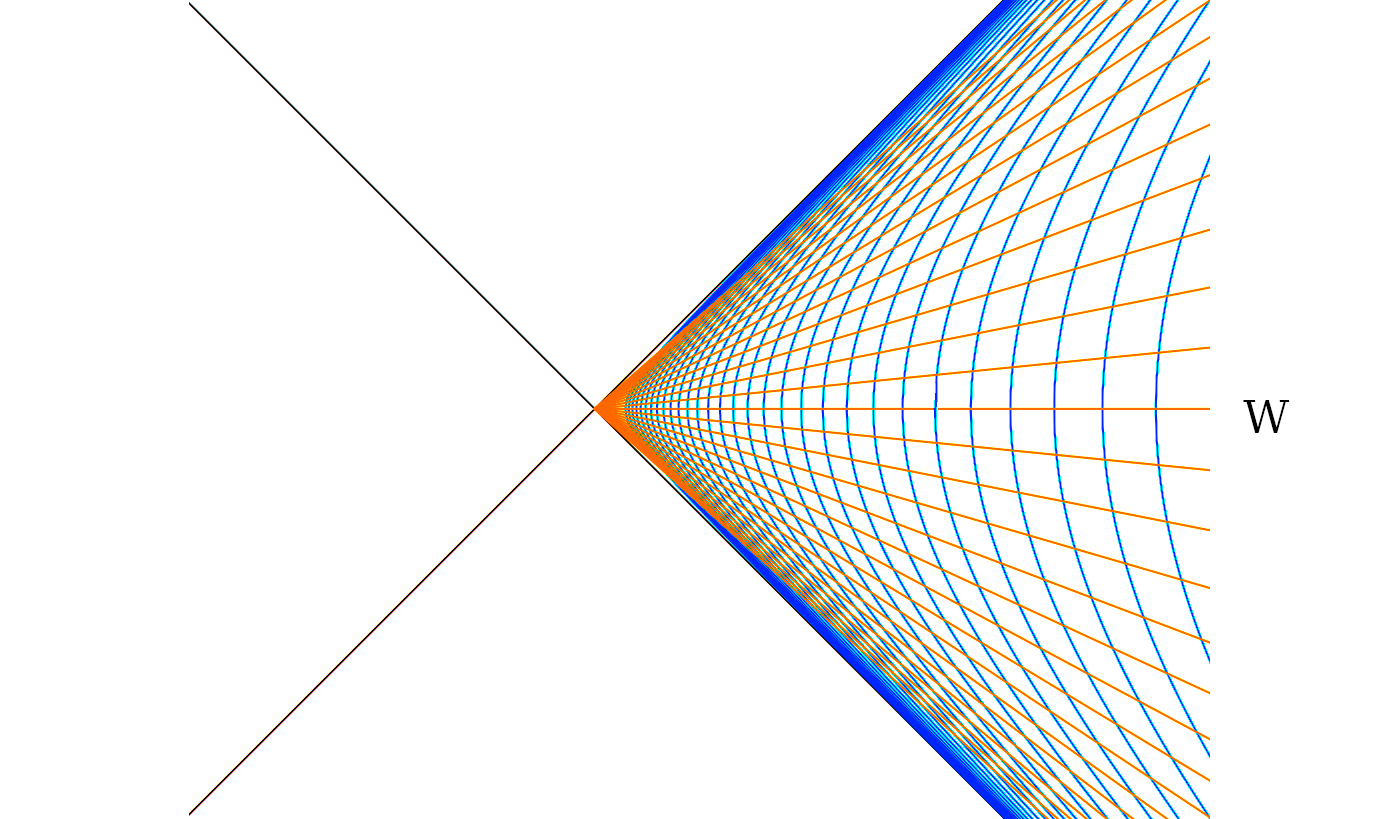
\includegraphics[scale=0.2]{rindler_w.png}
\caption{Rindler wedge $I$ on the right.}
\label{rindlerw}
\end{figure}

The massless Klein-Gordon equation in Rindler coordinates is
\begin{equation}
  \Box \phi = e^{-2a \xi}(-\partial_\eta^2 + \partial_\xi^2) \phi = 0
\end{equation}
The wave equation retains the same structure as the Minkowski case, up to the overall conformal factor $e^{-2a\xi}$. Since this factor does not affect the null structure of the equation, the mode solutions retain the same plane wave form in the Rindler time coordinate.
\begin{equation}
 r_k(\eta,\xi) = \frac{1}{\sqrt{4 \pi \omega_k}} e^{-i(\omega_k \eta -k \xi)} + \text{h.c.}
\end{equation}
for each wave number $k$ and positive frequency $\omega_k = |k| > 0$.  These ``Rindler modes'' are in terms of $\eta$ and $\xi$ and are thus confined to the Rindler wedge $W$.  Since Rindler coordinates only cover region I (the right wedge), these modes are not defined globally in Minkowski space. This leads to an inequivalence between the Minkowski and Rindler quantizations.

\subsection{Unruh Modes}
For $\omega_k = k > 0$, and
\begin{equation}
  \begin{array}{llll}
    \alpha_k &= \frac{e^{\frac{\pi\omega_k}{2a}}}{\sqrt{2 \sinh \frac{\pi \omega_k}{a}}} &= \sqrt{\frac{1}{1 - e^{-2\pi\omega_k / a}}} &  \\
    \beta_k &= \frac{e^{\frac{-\pi\omega_k}{2a}}}{\sqrt{2 \sinh \frac{\pi \omega_k}{a}}} &= \sqrt{\frac{1}{e^{2\pi\omega_k / a} - 1}} & \quad \text{(thermal form)} \\
  \end{array}
  \label{alpha_beta}
\end{equation}
noting that $\alpha_k^2 - \beta_k^2 = 1$. We analyticaly continue $r_k$, $r_{-k}$ to the $t,x$ plane as
\begin{equation}
  \begin{array}{ll}
    r_{+k} &= \frac{1}{\sqrt{4 \pi \omega_k}} e^{-i(\omega_k \eta - k \xi)} = \frac{1}{\sqrt{4 \pi \omega_k}} (a(-t + x + i \epsilon))^{\frac{i \omega_k}{a}} \\
    r_{-k} &= \frac{1}{\sqrt{4 \pi \omega_k}} e^{-i(\omega_k \eta + k \xi)} = \frac{1}{\sqrt{4 \pi \omega_k}} (a(-t - x + i \epsilon))^{\frac{-i \omega_k}{a}} \\
  \end{array}
\end{equation}
Define also
\begin{equation}
  \begin{array}{ll}
    \varphi_{+k} &= \frac{1}{\sqrt{4 \pi \omega_k}} e^{-i(\omega_k t - k x)}\\
    \varphi_{-k} &= \frac{1}{\sqrt{4 \pi \omega_k}} e^{-i(\omega_k t + k x)}\\
    \mu^R_k &= \alpha_k (r_k - r_{-k}^*) \\
    &= \frac{e^{\frac{\pi \omega_k}{2a}}}{\sqrt{2 \sinh \frac{\pi \omega_k}{a}}} \left(r_k - r_{-k}^* \right) \\
    &= \frac{1}{\sqrt{4 \pi \omega_k}\sqrt{2 \sinh \frac{\pi \omega_k}{a}}} \left( e^{\frac{\pi \omega_k}{2a}} \left(a(-t+x+i\epsilon)\right)^{\frac{i\omega_k}{a}} + e^{\frac{-\pi \omega_k}{2a}} \left(a(t+x-i\epsilon)\right)^{\frac{i\omega_k}{a}} \right) \\
    \mu^L_k &= \beta_k (r_k^* - r_{-k} )\\
    &=\frac{e^{\frac{-\pi \omega_k}{2a}}}{\sqrt{2 \sinh \frac{\pi \omega_k}{a}}} \left(r_k^* - r_{-k} \right) \\
    &=\frac{1}{\sqrt{4 \pi \omega_k}\sqrt{2 \sinh \frac{\pi \omega_k}{a}}} \left( e^{\frac{-\pi \omega_k}{2a}} \left(a(-t+x+i\epsilon)\right)^{\frac{-i\omega_k}{a}} + e^{\frac{\pi \omega_k}{2a}} \left(a(t+x-i\epsilon)\right)^{\frac{-i\omega_k}{a}} \right) \\
  \end{array}
\end{equation}
%TODO (verify U = r_k expressions)

\begin{figure}[h]
\centering
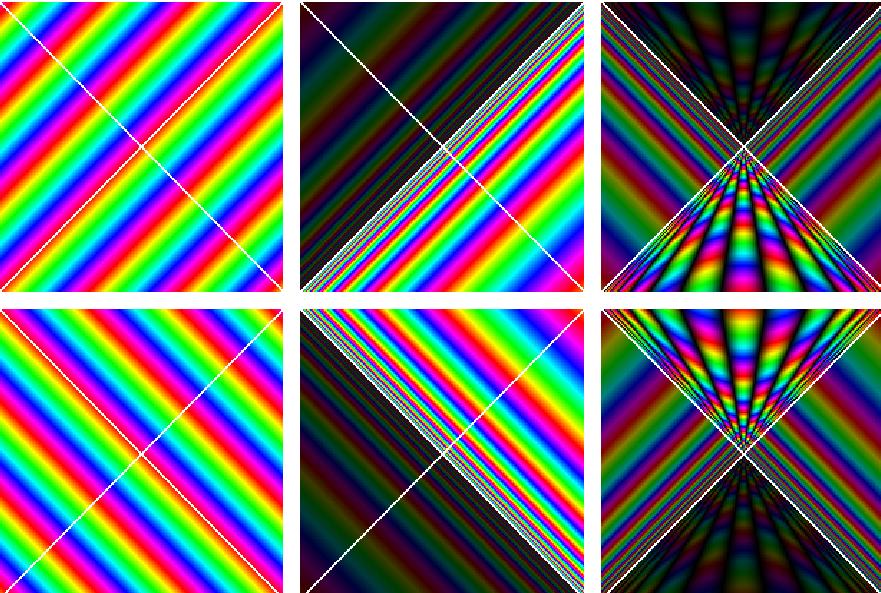
\includegraphics[scale=0.5]{unruh_mode_rainbow.png}
\captionsetup{width=0.9\textwidth}
\caption{Space time diagrams for $\left[\begin{array}{ccc} \varphi_k & r_k & \mu^R_k \\ \varphi_{-k} & r_{-k} & \mu^L_k \end{array} \right]$. Color represents phase; brightness shows magnitude. The consistent "rainbow" phase structure in $\varphi_k$ and $\mu_k$ reflects their pure positive frequency content in Minkowski time, unlike $r_k$, which varies across branches. The left moving Rindler modes $r_k$(top) correspond to emission and the right moving mode $r_{-k}$ (bottom) to absorption.}
\label{unruh_rainbow}
\end{figure}

\subsection{Bogoliubov Transforms}
Let the superscripts $(0)$, $(0c)$, $(M)$ etc represent frames of reference. We have a Bogoliubov transformation matrix from $M$ to $W_0$ of
\begin{equation}
  \left[ \begin{array}{l}
    a^{(0)}_k \\
    a^{(0)}_{-k} \\
    \hline
    a^{(0)\dagger}_k \\
    a^{(0)\dagger}_{-k} \\
 \end{array} \right] = 
  \left[
\begin{array}{rr|rr}
    \alpha_k &       0   &  0       & \beta_k \\
    0        & -\alpha_k & -\beta_k & 0 \\
    \hline
    0        & \beta_k   & \alpha_k & 0 \\
    -\beta_k &    0      &   0      & -\alpha_k \\
\end{array} \right]_{k,q}
\left[ \begin{array}{l}
    c^R_q \\
    c^L_q \\
    \hline
    c^{R\dagger}_q \\
    c^{L\dagger}_q \\
 \end{array} \right]
\end{equation}
for a change of basis from $a^{(M)}$ to $c^R$ and $c^L$
\begin{equation}
  \phi = \int \dv{q} \mu_q^R c_q^R + \mu_q^L c_q^L + \text{h.c.}
  \label{c_ladder}
\end{equation}
From this we compute the usual Unruh radiation equation with Planck spectrum (compare $\beta_k$ with equation (\ref{alpha_beta})) to obtain
\begin{equation}
  a_k^{(0)} = \alpha_k c_q^R + \beta_k c_q^{L\dagger}
\label{a_in_c}
\end{equation}

We compute the Bogoliubov coefficients for
\begin{equation}
  \begin{array}{ll}
  a^{(c)}_k &= \int \dv{q} \alpha^{(cM)}_{kq} a^{M}_q + \beta^{(cM)}_{kq} a^{(M)\dagger}_q \\
  &= \int \dv{q} \alpha^{(c0)}_{kq} a^{(0)}_q + \beta^{(c0)}_{kq} a^{(0)\dagger}_q
  \end{array}
\end{equation}
as
\begin{equation}
  \begin{array}{ccl}
    \alpha^{(cM)}_{kq} &= \left<\varphi_q, r_k^{(c)} \right> &= \frac{1}{a \pi} \sqrt{\frac{\omega_k}{\omega_q}} \left(\frac{a}{q}\right)^{\frac{i\omega_k}{a}} e^{\frac{\pi \omega_k}{a}} \Gamma\left(\frac{i\omega_k}{a}\right) \\
    \beta^{(cM)}_{kq} &= \left<\varphi_q^*, r_k^{(c)} \right> &= \frac{1}{a \pi} \sqrt{\frac{\omega_k}{\omega_q}} \left(\frac{a}{q}\right)^{\frac{-i\omega_k}{a}} e^{\frac{-\pi \omega_k}{a}} \Gamma\left(\frac{-i\omega_k}{a}\right) \\
    \alpha^{(c0)}_{kq} &= \left<r_q^{(0)}, r_k^{(c)} \right> &= \frac{1}{2 \pi a}\sqrt{\frac{\omega_k}{\omega_q}} (ac)^{\frac{-i(\omega_q - \omega_k)}{a}} B\left(\frac{i\omega_k}{a}, \frac{i(\omega_q - \omega_k)}{a}\right) \\
    \beta^{(c0)}_{kq} &= \left<r_q^{(0)*}, r_k^{(c)} \right> &= \frac{1}{2 \pi a}\sqrt{\frac{\omega_k}{\omega_q}} (ac)^{\frac{-i(\omega_q + \omega_k)}{a}} B\left(\frac{-i\omega_k}{a}, \frac{i(\omega_q + \omega_k)}{a}\right) \\
  \end{array}
  \label{bogo}
\end{equation}
We can compare absolute magnitudes for $M$ v.s. $W_c$ and see that they don't depend on $q$ or $c$
\begin{equation}
  \begin{array}{cc}
    \left|\beta_{kq}^{(c_1M)}\right|^2 = \left|\beta_{kq}^{(c_2M)}\right|^2 & \\
    \left|\beta_{kq}^{(c_1M)}\right|^2 = \left|\beta_{kq}^{(c_2M)}\right|^2 & \\
    \left|\beta_{kq}^{(cM)}\right|^2 / \left|\alpha_{kq}^{(cM)}\right|^2 = e^{\frac{-2\pi\omega_k}{a}}  & \text{   (thermal factor)} \\
 \end{array}
\end{equation}
The $c$ independence is expected since Unruh radiation is translation invariant. The $q$ independence can be strengthened as the expected number of particles in mode $k$
\begin{equation}
 \int \dv{q} \left|\beta_{kq}^{(cM)}\right|^2 = \frac{e^{\frac{-2 \pi \omega_k}{a}}}{2 \sinh \frac{\pi \omega_k}{a}} \int \dv{q} \frac{2}{a\pi |q|}
\end{equation}
where we factor out the divergent part to recover the radiation equation again.

We next turn to $W_c$ v.s. $W_0$ and also find $c$ independence there 
\begin{equation}
  \begin{array}{c}
    \left|\alpha_{kq}^{(0c_1)}\right| = \left|\alpha_{kq}^{(0c_2)}\right| \vspace{4pt}\\
    \left|\beta_{kq}^{(0c_1)}\right| = \left|\beta_{kq}^{(0c_2)}\right| \\
  \end{array}
\end{equation}
\begin{equation}
  \begin{array}{ll}
      \left|\beta_{kq}^{(0c)}\right|^2 / \left|\alpha_{kq}^{(0c)}\right|^2 \vspace{4pt} &= \left|\Gamma\left(\frac{i(\omega_q + \omega_k)}{a}\right)\right|^2 / \left|\Gamma\left(\frac{i(\omega_q - \omega_k)}{a}\right)\right|^2 \vspace{4pt} \\
  & = \frac{(\omega_q - \omega_k) \sinh \pi (\omega_q - \omega_k)}{(\omega_q + \omega_k) \sinh \pi (\omega_q + \omega_k)} \\
  \end{array}
  \label{nonzero_ratio}
\end{equation}
which is somewhat more surprising since this implies that $\int \dv{q} \left|\beta_{kq}^{(c_2c_1)}\right|^2$ is a $c_1$ and $c_2$ independent factor  for every shifted wedge inclusion.  In other words, the expected number of particles for a mode $r^{(c_2)}_k$ of $W_{c_2}$ in $W_{c_1}$'s vacuum is independent of the choice of shift $c_2$ and $c_1$.

More explicitly we have a transform matrix of $\Lambda_c$ from $W_0$ to $W_c$ 
\begin{equation}
  \left[ \begin{array}{l}
    a^{(c)}_k \\
    a^{(c)}_{-k} \\
    \hline
    a^{(c)\dagger}_k \\
    a^{(c)\dagger}_{-k} \\
 \end{array} \right] = \underbrace{
  \left[
\begin{array}{rr|rr}
    A_c        &       0   &  B_c            &  0 \\
    0        &      -A_c   &  0            & -B_c \\
    \hline
    \overline{B_c}        &    0      &  \overline{A_c} & 0 \\
    0 &    -\overline{B_c}      &   0           & -\overline{A_c} \\
\end{array} \right]_{k,q} }_{\Lambda_c}
  \left[ \begin{array}{l}
    a^{(0)}_q \\
    a^{(0)}_{-q} \\
    \hline
    a^{(0)\dagger}_q \\
    a^{(0)\dagger}_{-q} \\
 \end{array} \right]
\end{equation}
where $A_c = \alpha_{kq}^{(c0)} = P_c A_1 P_c^{-1}$  and $B_c = \beta_{kq}^{(c0)} = P_c B_1 P_c$ for a diagonal phase factor matrix
\begin{equation}
  P_c = P_{c,rs} = \delta(r - s) c^{\frac{i\omega_r}{a}} = e^{\frac{i H}{a} \log c}
\end{equation}
We can write $\Lambda_c$ out compactly out as
\begin{equation}
  \Lambda_c = Q_c \Lambda_1 Q_c^{-1}
\end{equation}
where
\begin{equation}
  Q_c = \left[\begin{array}{cccc}
        P_c, & 0 & 0 & 0 \\
        0 & P_c & 0 & 0 \\
        0 & 0 & P_c^{-1} & 0 \\
        0 & 0 & 0 & P_c^{-1} \\
    \end{array} \right] 
\end{equation}
Note that $\lim_{c\to 0} \Lambda_c = 1$ since the limit of $\lim_{c\to 0} \alpha_{kq}^{(c0)} = 1$ and $\lim_{c\to 0} \beta_{kq}^{(c0)} = 0$, which corresponds nicely to $\lim_{c\to 0} W_c = W_0$. The composition of Bogoliubov transforms, $\Lambda_{nc} = \Lambda_c^n$, yields
\begin{equation}
  \begin{array}{ll}    
    Q_{nc} \Lambda_1 Q_{nc}^{-1}  &= \Lambda_{nc} \\
         &= \left(Q_c \Lambda_{c} Q_c\right) \left( Q_c^{-1} \Lambda_{c} Q_c\right) \cdots \left(Q_c \Lambda_{c} Q_c\right) \\
  &= Q_c \Lambda_c^n Q_c^{-1} \\
  \end{array}
\end{equation}
so that
\begin{equation}
  \begin{array}{ll}
  \Lambda_c^n &= Q_c^{-1} Q_{nc} \Lambda_1 Q_{nc}^{-1} Q{c} \\
  &= Q_n \Lambda_1 Q_n^{-1}
  \end{array}
\end{equation}
and more generally we have a one parameter group given by
\begin{equation}
  \left\{\Lambda_0^x = Q_x \Lambda_0 Q_x^{-1} : x \in \mathbb{R} \right\}.
\end{equation}
These Bogoliubov transformations between shifted wedges define a one-parameter group, reflecting an underlying symmetry structure. This naturally connects to modular flow as studied in algebraic QFT, where such transformations correspond to automorphisms generated by the modular operator. This is an explicit realization of modular flow, due to the von Neumann algebra modular automorphism associated with the translation $W_0 \rightarrow W_c$, studied in detail in Tomita-Takesaki theory \cite{Borchers2000}.  There we find thermal KMS states between open set inclusions in a much more general setting.


Consider a sequence
\begin{equation}
  W_{c_n} \subseteq \cdots \subseteq W_{c_i} \subseteq \cdots \subseteq W_{c_j} \subseteq W_{c_2} \subseteq W_{c_1}
\end{equation}
Then each $W_{c_i} \subseteq W_{c_j}$ involves particle production with a fixed squared magnitude for mode $k$.  We calculate this expected number of $W_{c_i}$ particles for mode $k$ in $W_{c_j}$'s vacuum
\begin{equation}
  \bra{0_{W_{c_j}}} a^{(c_i)\dagger}_k a^{(c_i)}_k \ket{0_{W_{c_j}}} = \frac{1}{2 \pi^2 k \sinh \frac{\pi k}{a}} \int_{x=0}^\infty \frac{x \sinh x}{(x+\frac{\pi k}{a}) \sinh(x+\frac{\pi k}{a})}
\end{equation}
which diverges.  The integrand goes to $e^{-\frac{\pi k}{a}}$ as $x$ gets large, so we can see that the expected number of particles in ratio goes to
\begin{equation}
  \frac{1}{m (e^{2m} + 1)} = \frac{1}{k (e^{\frac{2\pi \omega_k}{a}} - 1)}.
\end{equation}

\section{Driving Sources}

We now ask a fundamental question: {\bf ``What exactly is accelerating the observer?''} Until this point, we've treated acceleration as a coordinate choice, without invoking any underlying physical mechanism. We have also not specified the observer’s precise location within the Rindler wedge, nor the spatial origin of the observed excitations. These ambiguities reflect the effective coarse-graining over the observer's details, a feature that contributes to the thermal character of the Unruh effect.

Figure \ref{emit_absorb} illustrates the situation for a sharply peaked frequency wave packet made of Rindler modes. The modes $r_k$ are left-moving, propagating toward the future horizon and are interpreted as {\bf emission}. The $r_{-k}$ modes are right-moving, originating from the past horizon and are interpreted as {\bf absorption}. The Rindler modes are constructed as superpositions of Minkowski modes $\varphi_q$, effectively smeared over a range of frequencies. This is visually evident in Figure \ref{unruh_rainbow}, where the local frequencies increase (blue-shift) near the horizons. This is made explicitly by the Bogoliubov coefficients $\alpha_{kq}^{(cM)}$ and $\beta_{kq}^{(cM)}$ which encode the Fourier decomposition of the Rindler modes through their Klein-Gordon inner products with the Minkowski modes $\varphi_q$ and $\varphi_q^*$, respectively. This frequency delocalization, tied to the observer's acceleration horizon, underlies the apparent thermal character of the radiation.

\begin{figure}[h]
\centering
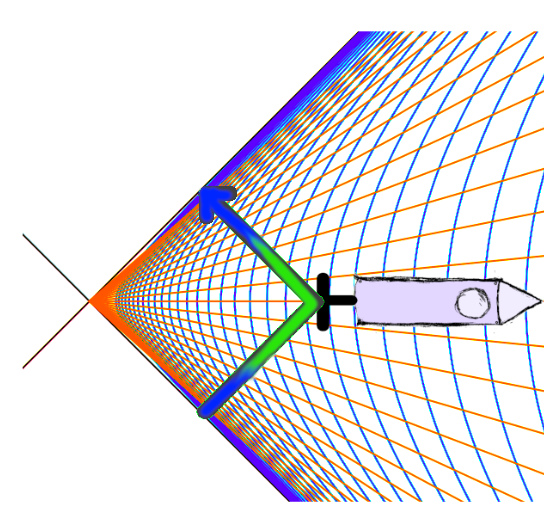
\includegraphics[scale=1.5]{emit_absorb.png}
\captionsetup{width=0.7\textwidth}
\caption{
  A Rindler mode's frequency is smeared out in Minkowski space, blue-shifted near the horizon. We diagram a particle as if it were striking a mirror at the rear of a rocket, where its reflection emerges as a combination of emission and absorption processes in the Rindler frame.}
\label{emit_absorb}
\end{figure}

To address this, we introduce a driving source, a physical mechanism responsible for the field's excitation and, indirectly, for the observer's acceleration. This reframes the interpretation: the radiation is not spontaneous but instead emerges as a coherent response to the source. The apparent thermality, then, is tied to our ignorance of the source's detailed structure.

We aim to encode the effect of a creation operator by introducing a source term $J(x)$ into the Lagrangian at some distant time in the past, which directly excites the field in a specific mode. Since $J(x)$ couples linearly, it prepares a coherent state that excites the chosen mode in a controlled, phase-coherent manner. To replicate the action of a creation operator, the source must be engineered such that its overlap with the mode functions $u_k(x)$ matches the operator’s action on the field.

The field can be expanded as in equation (\ref{c_ladder}), and the $\beta_k$-term in equation (\ref{a_in_c}) is responsible for the thermal particle content of the Minkowski vacuum as seen by Rindler observers. Without loss of generality\footnote{We only consider a fixed frequency and the $L$-mode, and extend the argument linearly to any positive frequency Minkowski modes.}, we encode the effect of a creation operator $c_k^{L \dagger}$ using
\begin{equation}
  c _k^{L\dagger} = \left<\phi, \mu_k^{L*}\right>_{KG} = \int \dv{x} \mu_k^{L*}(x) \phi(x)
\end{equation}
and the orthogonality of the mode functions in the Klein-Gordon inner product. In the generating functional formalism, setting $J_k^L(x) = -\beta_k u_k^{L*}$ the functional derivative $\frac{\delta}{\delta J_k^L}Z[J_k^L]|_{J_k^L=0}$ inserts $\phi$ into time-ordered correlators. Smearing this field insertion against $\mu_k^{L*}(x)$ thus projects onto $c_k^{L\dagger}$ and we have\footnote{The remaining $\alpha_k$ factor reflects the mismatch between the squeezed Unruh vacuum and the coherent state prepared by the source.}
\begin{equation}
\begin{array}{ll}
  a_k^{(0)J} &= \alpha_k c_q^R + \beta_k c_q^{L\dagger} -  \beta_k c_q^{L\dagger} \\
  &= \alpha_k c_q^R
\end{array}
\end{equation}

In Rindler coordinates, this source term prepares a modified field state in which the Rindler mode occupation differs from the thermal distribution of the Minkowski vacuum. Rather than simply adding energy, the source introduces a coherent excitation that cancels the mode structure induced by the Bogoliubov $\beta$-terms, effectively replacing their contribution. This lets us construct a state where the Rindler response is vacuum-like for mode k

\begin{equation}
  \bra{J_k^L}  b_k^{\dagger} b_k \ket{J_k^L} = \bra{0_M}  b_k^{J_k^L \dagger} b^{J_k^L}_k \ket{0_M} = 0
\end{equation}

\section{Localization}

Consider the two wedges $W_0$ and $W_c$ shown in Figure \ref{restrict}.  The grayscale part is the Rindler mode $r_q$ of $W_0$ (analytically continued to $M$).  The rainbow piece is $r_q$ restricted to $W_c$.  This restriction is missing the higher frequencies of $r_q$ that occur near the future event horizon\footnote{The same thing happens for $r_{-q}$ but with the past event horizon instead.}.

\begin{figure}[h]
  \centering
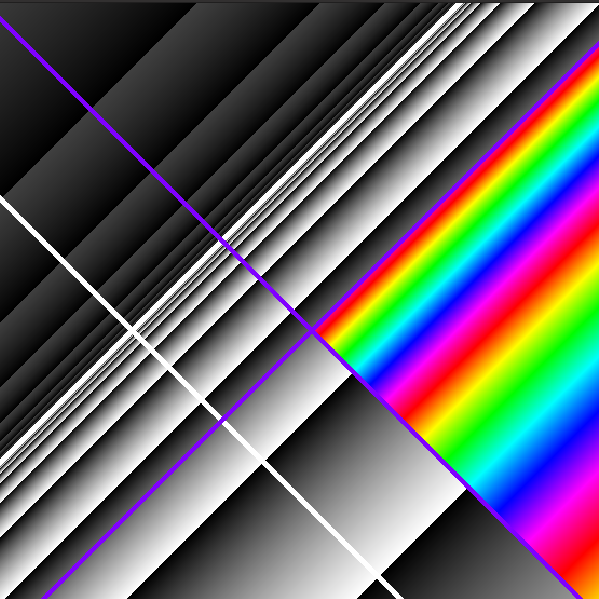
\includegraphics[scale=0.3]{wedge_in_wedge.png}
\caption{A Wedge $W_c$ (blue) inside of the wedge $W_0$ (red). Rindler mode $r_q$ of $W_0$ (grayscale) restricted to $W_c$ (rainbow).}
\label{restrict}
\end{figure}

We have somewhat localized $r_q$ by considering its restriction to $W_c$.  The localization is not complete, the observer can still be anywhere within the wedge $W_c$, but we have at least isolated it from the wild oscillations of $r_q$ near the $W_0$ horizons. To further study the situation, consider $\alpha^{(c0)}_{kq}$ from equation (\ref{bogo}).  We fix $q$ and find that
\begin{equation}
  \left|\left<r_q^{(0)}, r_k^{(c)} \right>\right|^2 = \frac{\sinh \frac{\pi \omega_q}{a}}{4\pi a \sinh \frac{\pi \omega_k}{a} (\omega_q - \omega_k) \sinh \frac{\omega_q - \omega_k}{a}}
\end{equation}
See Figure $\ref{peaked}$, where we now find a peaked response at $\omega_k = \omega_q$.  We still find the thermal term from before $\sinh \frac{\pi \omega_k}{a}$ contributing a spread near $\omega_k = 0$ and the $(\omega_q - \omega_k) \sinh \frac{\omega_q - \omega_k}{a}$ near the peak at $\omega_k = \omega_q$, but the large scale peaked response itself is due to the localization.

\begin{figure}[h]
  \centering
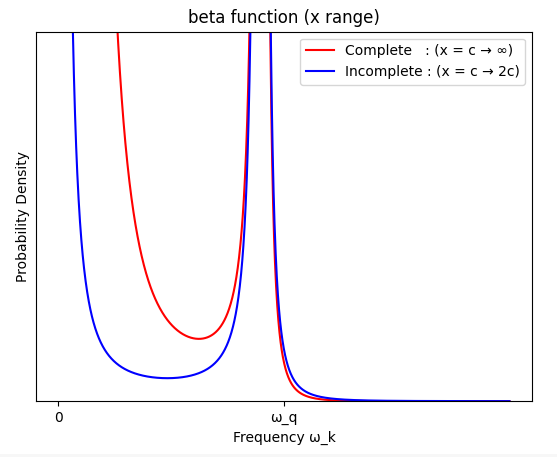
\includegraphics[scale=0.6]{peaked.png}
\caption{The Rindler modes $r_k$ of $W_c$ have peaked spectral response to $r_k$ at $\omega_k = \omega_q$.}
\label{peaked}
\end{figure}


\section{Appendix Formulas}
Some useful formula
\begin{equation}
  \int_{c}^\infty x^a (x-c)^b \dv{x} = c^{a+b+1} B(b+1, -a-b-1)
\end{equation}
TODO, check this next one
\begin{equation}
  \int_{-\infty}^\infty e^{ikx} x^b \dv{x} = -\frac{2i}{k^{b+1}} e^{\frac{-\pi b}{2}} \Gamma(b+1)
\end{equation}
This is useful for the shifted wedge inner products. Let
\begin{equation}
  f_{k,b,d} = \left(a\left(b(t-i\epsilon)+x\right)\right)^\frac{id\omega_k}{a}
\end{equation}
Then
\begin{equation}
  \left< f_{k,b_k,d_k}, f_{q,d_q,d_q}\right> = \frac{1}{2\pi} \sqrt{\frac{\omega_k}{\omega_q}} (ac)^\frac{i(d_k\omega_k - d_q \omega_q)}{a} \left((-d_k)\frac{b_k + b_q}{2} \right) B\left(\frac{id_k\omega_k}{a}, \frac{-i(d_k\omega_k - d_q \omega_q)}{a}\right)
\end{equation}
We frequently use
\begin{equation}
  |\Gamma(ib)|^2 = \frac{\pi}{b \sinh \pi b}
\end{equation}


\section{Conclusion and Prediction}
If the thrust required to accelerate a detector is not explicitly accounted for, it manifests instead as an apparent thermal feature of the vacuum—Unruh radiation. However, as demonstrated in this paper, Unruh radiation can be directly explained as a consequence of thrust. This perspective leads to the prediction that neither Unruh radiation nor Hawking-Bekenstein radiation should appear independently of the thrust that drives the system.

\begin{figure}[h]
\centering
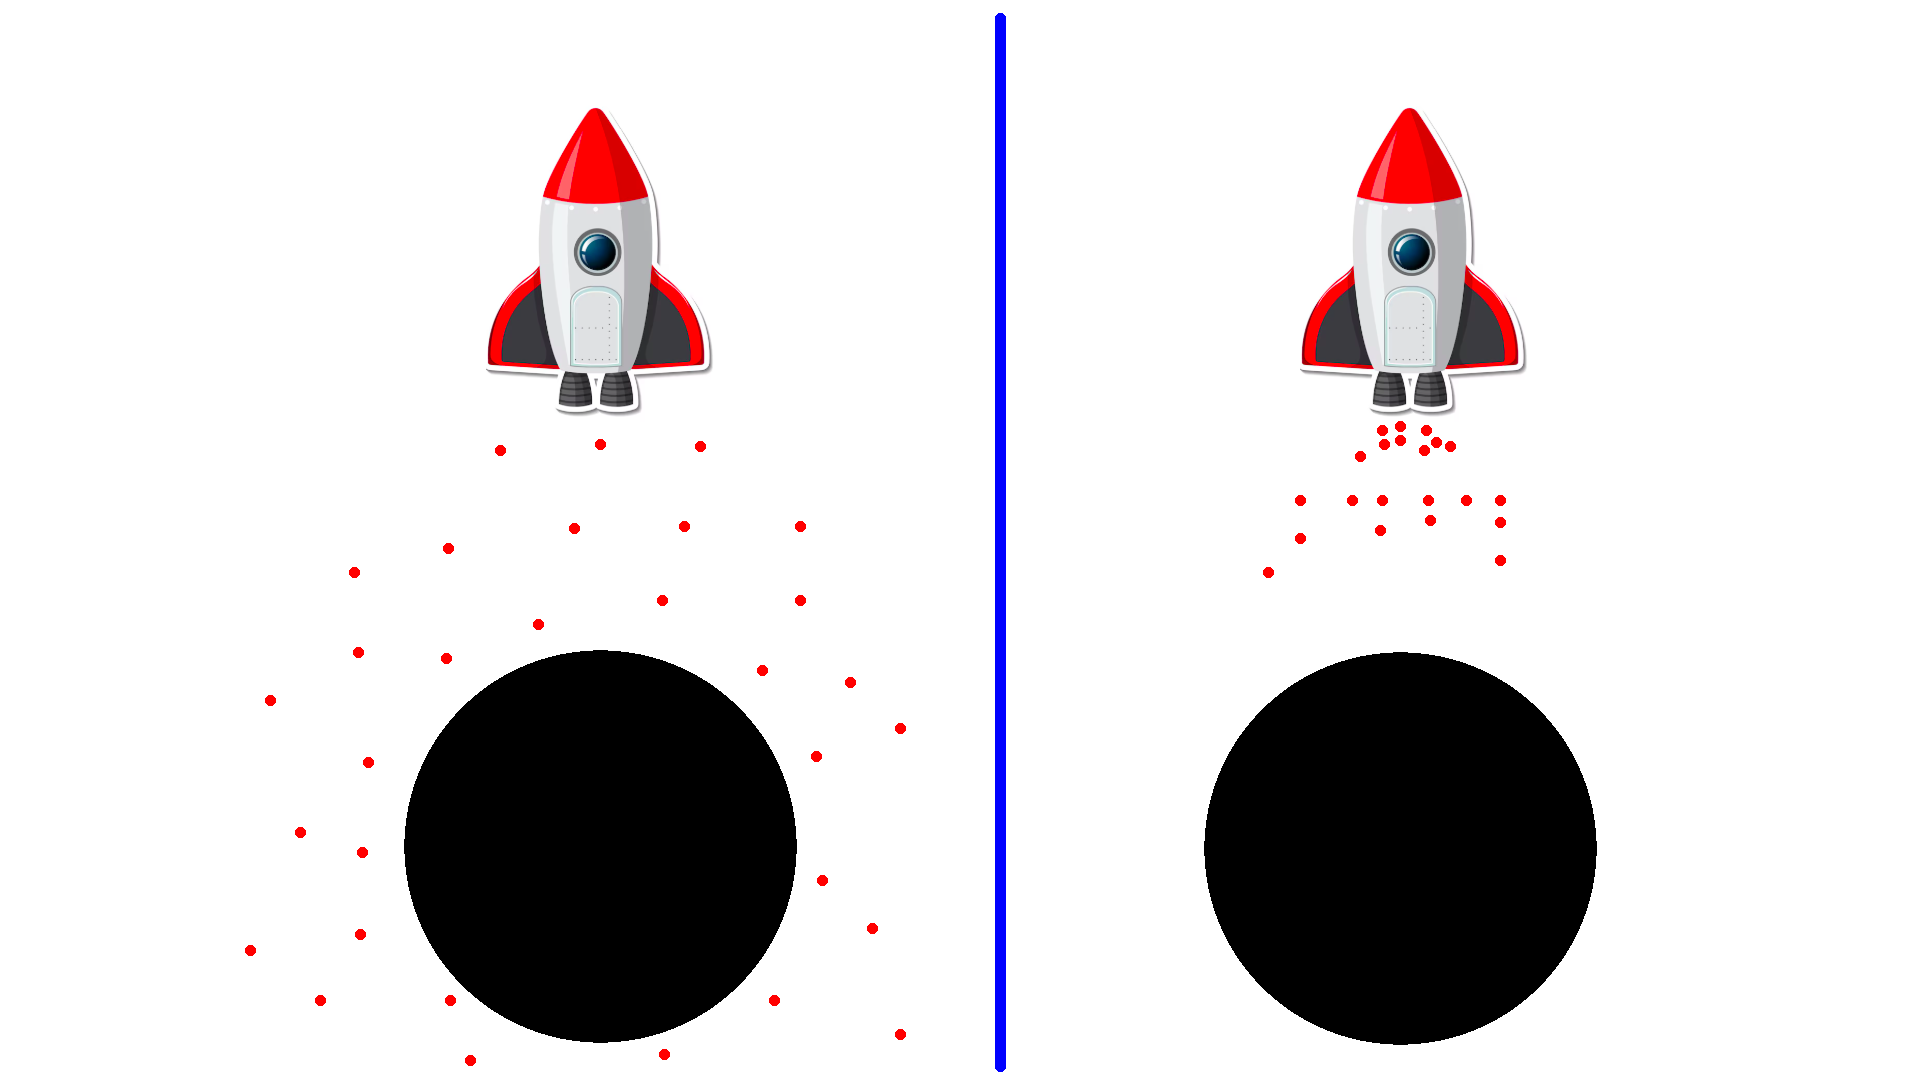
\includegraphics[scale=0.5]{rocket.png}
\caption{Hawking picture of black hole radiating on the left. Our picture of a rocket thrusting on the right.}
\label{rocket}
\end{figure}

\section{Acknowledgments}
Thanks to Ben Commeau and Daniel Justice for useful discussions.

\bibliographystyle{ieeetr}
\bibliography{bibliography}

\end{document}
